\documentclass[letterpaper,twocolumn,10pt]{article}
\usepackage{usenix,epsfig}
\usepackage{xcolor}
\usepackage{listings}
\usepackage[]{algorithm2e}
\usepackage{changepage}
\usepackage{hyperref}
\definecolor{mygreen}{rgb}{0.1,0.5,0.1}
\definecolor{myblue}{rgb}{0.1,0.1,0.7}

\hypersetup{
    colorlinks,
    linkcolor={red!50!black},
    citecolor={blue!50!black},
    urlcolor={blue!80!black}
}

\lstset{language=C,
    basicstyle=\footnotesize\ttfamily,
    keywordstyle=\color{myblue}\ttfamily,
    stringstyle=\color{mygreen}\ttfamily,
    commentstyle=\color{gray}\ttfamily,
    keepspaces=true,
    tabsize=2,
    otherkeywords={bool}
}

\newcommand{\code}[1]{\lstinline{#1}}
\newcommand{\vignat}{{\sc VigNAT}\xspace}
\newcommand{\vignata}{{\sc VigNAT$\alpha$}\xspace}
\newcommand{\vignatb}{{\sc VigNAT$\beta$}\xspace}

\newcommand{\todo}[1]{\textcolor{red}{TODO: #1}}

\newcounter{solOverviewSteps}

\begin{document}

%don't want date printed
\date{}

%make title bold and 14 pt font (Latex default is non-bold, 16 pt)
\title{\Large \bf Vigor: Toward Carrier-Grade Software Network Functions}

%\author{
%    {\rm Arseniy Zaostrovnykh}\\
%    EPFL
%    \and
%    {\rm Katerina Argyraki}\\
%    EPFL
%    \and
%    {\rm George Candea}\\
%    EPFL
%}
\author{
    {\rm Paper \#113}\\
}

\maketitle

% Use the following at camera-ready time to suppress page numbers.
% Comment it out when you first submit the paper for review.
\thispagestyle{empty}


\subsection*{Abstract}
The objective of this work is to enable developers to productively write software-based data plane network functions that simultaneously meet the highest standards of reliability, security, and performance. We present a verification approach for formally proving properties of stateful network functions, in a way that is practical both in terms of developer effort and the performance of the resulting data plane software. Unlike alternative approaches that require drastic changes in the way network functions are developed, our approach allows the use of C/C++ together with popular frameworks like DPDK. To the best of our knowledge, our work is the first to both be practical and formally verify stateful network functions. We introduce a new ``speculative'' form of symbolic execution, which achieves scalability to real-world network functions by leveraging insights related to the structure and cyclomatic complexity of data plane software. This technique dovetails with a new library of verified components that are commonly used in network functions. We illustrate our approach by developing a middlebox that is verified to never crash, to not leak memory, be free of several classes of security vulnerabilities, and whose performance is on par with other NATs. %\footnote{Disclaimer: we use acronym NAT in this paper to refer to a more narrow kind - Dynamic Source NAPT (network address-port translation~\cite{rfc3022}).}. 
We view this as an important milestone on the road to complete verification of all software-based network functions.

\section{Introduction}

Product development in the telecommunication industry has traditionally followed rigorous standards for quality, security, and protocol adherence, with the term carrier-grade designating network equipment that meets these high standards. While this model worked well in the past, it typically entailed reliance on proprietary hardware and long product cycles, which slowed progress. To meet the growing demand for new network functionality and faster deployment cycles, network service providers started turning to software.

In recent years, new platforms emerged for developing network functionality in software~\cite{kohler2000click,bosshart2014p4,mccanne1993bsd,song2015unified,shah2003np,shahbaz2016pisces}, enabling the rapid prototyping and deployment of new routing protocols~\cite{sivaraman2016packet}, QoS policies~\cite{sivaraman2016programmable}, load balancing algorithms~\cite{zhang2013steering}, intrusion prevention systems~\cite{xing2014sdnips}, etc. The agility that software engenders determined even traditional hardware-based network device manufacturers to invest in software-based approaches~\cite{ciscodevelopssdn}.

But this raises the question of how to develop carrier-grade network functions (NF) in software? Since NFs are often part of critical infrastructure, they must simultaneously be secure, reliable, and high-performance, i.e., be carrier-grade. The Achilles' heel of software has always been the (perceived) lack of reliability and security, particularly when it is written in C. This has led researchers to advocate using safe languages~\cite{clipsham2015safe, kourtis2015intelligent, fowler2014verified} or relatively heavyweight approaches~\cite{madhavapeddy2007melange, madhavapeddy2005splat, musuvathi2004model, alur2001verifying, ennals2004linear, ridge2008rigorous, qadir2015applying}. Yet many frameworks (e.g., P4~\cite{bosshart2014p4}, DPDK~\cite{intel2014data}, PF\_RING~\cite{pfring}, NetMap~\cite{rizzo2012revisiting}) and standalone implementations (Open vSwitch~\cite{pfaff2009extending}, NetFilter~\cite{boye2013netfilter}) use C. % These approaches require developers to drastically change or augment the way in which they write these network apps: massively annotate their code with logical derivations, use ``pure'' (side-effect-free) functions, abandon manual memory management and layout, and/or learn a new language.

Developers do not want to change the way they write code, they want to be able to convince their users that the code they wrote is carrier-grade (and, if they cannot prove correctness, to then fix the corner cases that impede the proof). We conducted a small survey~\cite{verifsurvey} among NF developers from both industry and academia, and almost 70\% insist on continuing to use C. % instead of a higher level alternative. With current common practices and languages, it is not possible to achieve the desired level of confidence. The continued perception of unreliability and insecurity hinders adoption and therefore slows down progress (can we quote an operator who doesn't want to deploy stuff out of fear?).

The goal of our work is to enable developers to provide  carrier-grade network functionality in software without having to do a forklift upgrade of their programming practices. In this paper we present a technique and a tool suite (a) for formally verifying crash- and leak-freedom as well as the absence of several classes of security vulnerabilities in NFs written in C/C++ (b) in a way that is practical both in terms of developer effort and the performance of the resulting software.

There exist approaches for providing formal guarantees for {\em stateless} network packet processing code~\cite{dobrescu2014software}; to the best of our knowledge, we are the first to provide such guarantees for real-world {\em stateful} software NFs without impacting performance. There are many such NFs: all dynamic routing protocols (RIP, BGP, STP), NAT, BRAS~\cite{wiki:bras}, CDN, IDS, DPI boxes, etc.

Practical verification of stateful software NFs is a difficult research problem. Hence none of the verification techniques proposed so far can scale anywhere close to verifying real-world stateful NFs. For the purpose of this paper, we take as an objective to develop a NAT~\cite{rfc3022} box that is proven to not have certain classes of vulnerabilities or crash or hang under any input. Even though NAT is a classic network function, it has proven hard to get right over time: the NAT on various Cisco devices can be crashed~\cite{cve-2015-6271} or hung~\cite{cve-2013-1138} by carefully crafted inputs, with the same type of problems existing in Juniper's NAT~ \cite{cve-2014-3817}, NATs based on NetFilter~\cite{cve-2014-9715}, and the NAT in Windows Server~\cite{ms13-064}. Thus, a NAT function that is formally verified to not crash, while providing production-class performance, is an important milestone in this line of work.

We achieve both scalable verification and minimal developer effort by leveraging two insights into the verification of data plane software:
\begin{itemize}
    \item {\bf Canonical data structures}: Unlike general-purpose software, data plane software employs a small number of commonly used network data structures (hash table, least-prefix-match, rings, etc.) and components. These lend themselves naturally to being abstracted into a library. They can be formally verified a priori, and their proofs then automatically leveraged for proving properties of the code that uses them.
    \item {\bf Hybrid verification}: While typically one picks a verification technique and applies it throughout, any {\em one} technique works well for {\em some} of the code and not for other. However, data plane software offers us the opportunity to advantageously employ symbolic execution for high-level code (which is mostly stateless and has short execution paths) and verification based on separation logic to the library of components/data structures (which is highly stateful).
     
\end{itemize}

In this paper we present work that builds upon these insights and makes three contributions:
\begin{itemize}
    \item {\bf Speculative data plane verification} (SDPV), a technique for verifying stateful software NFs by fusing powerful formal verification with automatic symbolic execution. % It uses formal verification for data structures. It replaces them with simple models that encode some assumptions about the behaviour of the data structures. It then runs SE on the application code and later validates the used models. This approach postpones high-effort/low-return work and discards it when it turns out to be irrelevant.
    \item {\bf The Vigor library of verified components} along with a tool chain
      that makes SDPV available to those who write software NFs in C/C++.
      The library consists of data structures (Hash Map, Batcher, Static Array) and a Port Allocator that are common for software NF. % The tool-chain brings together existing SE and formal verification engines to test the proposed technique.
    \item {\bf The \vignat verified NAT box} that offers both high performance and is formally proven to not crash or leak memory. We estimate that it would take an NF developer about 1 week to develop and verify a NAT using Vigor.
\end{itemize}

In the rest of the paper, we give a short overview of Vigor (\S\ref{sec:solution-overview}), describe our design (\S\ref{sec:design}), and present our implementation (\S\ref{sec:implementation}). We then evaluate the technique for two NAT prototypes (\S\ref{sec:evaluation}), discuss limitations (\S\ref{sec:limitations}), present related work (\S\ref{sec:related-work}), and conclude (\S\ref{sec:conclusion}).

%==============================================

\section{Solution Overview}
\label{sec:solution-overview}

This section motivates and explains at a high level what it's like to use Vigor when developing NFs. For the sake of illustration, say we wish to develop a trivial stateful NF that implements the discard protocol~\cite{rfc863}: an infinite loop receives packets from one interface, discards the ones that go to port 9 (``discard port''), and forwards the others through another interface.

\begin{lstlisting}
#define CAP 512

int main() {
  struct packet packets[CAP] = {};
  int begin = 0, end = 0;

  while(1) {
    if (end != (begin - 1) || 
        !(end == CAP - 1 && begin == 0)) {
      if (receive_packet(&packets[end]) && 
          packets[end].port != 9)
        end = (end + 1)%CAP;
    }
    if (end != begin && can_send_packet()) {
      send_packet(&packets[begin]);
      begin = (begin + 1)%CAP;
    }
  }
  return 0;
}

\end{lstlisting}

In order to absorb bursts, the code employs a ring buffer. The interface to the
network is: \code{bool receive_packet(struct packet* dst)}, which
non-blockingly reads an inbound packet and stores it at \code{dst}, returning success or failure; \code{bool can_send_packet()}, which checks if a new packet can be sent; and \code{void send_packet(struct packet* src)}, which sends the packet stored at \code{src}. The application follows common practice: it consists of a main event loop, it has no other complex loops, and it uses a ring, a popular data structure in network programming.

To verify that this NF does not crash, one could use the approach in Dobrescu et al.~\cite{dobrescu2014software} and run exhaustive symbolic execution. The symbolic execution (SE) technique entails using a symbolic execution engine (SEE) to explore all paths through the code and check whether any failure conditions hold --- in our case crash conditions. The inputs to the program are marked ``symbolic,'' meaning that they subsume all possible input values, and then the SEE simulates the execution of the program while propagating the symbolic inputs along the dataflow paths into the program's variables. When facing a branch (e.g., an \code{if} or a \code{for} loop), the SEE clones the program state and takes each feasible path separately. Branches impose constraints on variable values (e.g., an \code{if} statement imposes restrictions on the values of the condition variable along the \code{else} branch); the SEE collects these constraints along each path. When evaluating a branch condition, the SEE asks an SMT constraint solver which of the branches are feasible, given the constraints collected so far on that path prefix.

One could use an SEE like KLEE~\cite{cadar2008klee} to symbolically execute the code above exhaustively --- once all paths are found to be crash-free, the crash-freedom proof is complete. To perform SE, it is necessary to provide symbolic models for the three network calls. Something simple suffices, such as \code{receive_packet} generating a new symbolic packet in \code{dst}; \code{can_send_packet} forking program state into two states, one for each possible return value; and \code{send_packet} doing nothing. 

Alas, symbolic execution would never terminate. The reason is ``path explosion'': there is a large (often infinite) number of paths to explore, so the SEE cannot finish.  Path explosion results from cyclomatic complexity~\cite{mccabe:cyclomatic}: every branch condition doubles the number of paths, and every loop multiplies it by a factor; in our case, three \code{if} conditions inside an infinite loop give rise to an infinite number of paths. 

{\bf Step 1: Add loop invariants.} Infinite (or very long) loops can be simplified using loop invariants~\cite[\S~2.1]{cormen2009introduction}. These are annotations that inform the SEE about invariant properties of the loop, such as ``no element of \code{packets} between \code{begin} and \code{end} has destination port equal to 9'', and are a good match for NF-style loops.  We added to KLEE support for havoc-ing~\cite{boogie} automatically, to take advantage of such invariants and essentially reduce the infinite loop to a single abstract iteration that can be reasoned about in one pass.
 
This change makes SE feasible, albeit impractical: for \code{CAP=5}, it takes 10 sec to exhaustively SE the code; for \code{CAP=30} it takes 15 min, for \code{CAP=60} it takes 3 hours, and so on. It takes long due to another classic SE challenge, ``symbolic indexing''~\cite{sen2005cute,godefroid2008automated,boonstoppel2008rwset}: when indexing an array with a symbolic variable (or when dereferencing a symbolic pointer), the constraints on program state become extremely complex, because the symbolic pointer or index could be referencing many different possible locations. The complexity of the constraints chokes the SMT solver, and the SEE grinds to a halt. In general, SE doesn't work for code with symbolic pointers or offsets. Alas, stateful C code almost always has some of these.

{\bf Step 2: Use abstract data structures.} In Vigor, we eliminate the problem of symbolic indexing by encapsulating program state into well-defined data structures and putting them into a ``library of components''. This works well for NF development, because the NF code uses a relatively small set of standard structures, such as ring buffers, hash tables, least-prefix-match tables, etc. We provide to the SEE symbolic models of these abstracted components that ``hide'' symbolic indexes and pointers from the SEE.

For our example, the library provides a \code{ring} with a simple interface: \code{bool ring_empty()} checks whether there is a packet in the ring, \code{bool ring_full()} checks whether the ring has run out of space, \code{void ring_push_back(struct packet* src)} adds packet \code{src} to the ring, and \code{void ring_pop_front(struct packet* dst)} removes a packet from the ring and places it in \code{dst}. We then write a symbolic model for the \code{ring} and provide it to the SEE instead of the actual implementation. The NF now becomes:

% \begin{lstlisting}
% bool ring_full() {return SYMBOLIC("full");}

% bool ring_empty() {return SYMBOLIC("empty");}

% void ring_push_back(struct packet* p) {
%   ASSERT(p->port != 9); //Extra check.
% }

% void ring_pop_front(struct packet* p) {
%   FILL_SYMBOLIC(p, sizeof(struct packet), 
%                 "popped_packet");
%   ASSUME(p->port != 9);
% }
% \end{lstlisting}

\begin{lstlisting}
#define CAP 512

int main() {
  struct packet p;
  while(LOOP(1)) {
    if (!ring_full())
      if (receive_packet(&p) && p.port != 9)
        ring_push_back(&p);
    if (!ring_empty() && can_send_packet()) {
      ring_pop_front(&p);
      ASSERT(p.port != 9);
      send_packet(&p);
    }
  }
  return 0;
}
\end{lstlisting}

Now exhaustive SE of the code takes less than 100 millisec with our modified
KLEE, regardless of the size of \code{CAP}.  The fact that the code does not
crash on any path amounts to a proof of crash freedom. Or does it? The validity
of the proof depends on (1)  our library implementation of \code{ring} not
crashing; and (2) the symbolic model of \code{ring} accurately capturing how the
\code{ring} implementation works ({\em Step 3}).

Suppose we had an overapproximate model:
\begin{lstlisting}
void ring_pop_front(struct ring* r,
                    struct packet* p) {
  FILL_SYMBOLIC(p, sizeof(struct packet),
                "popped_packet");
}
\end{lstlisting}
Then the \code{ASSERT} from the previous listing would fail.

The Vigor library comes with a formal specification and a formal proof that the implementation satisfies that specification. In other words, there is a formal spec for \code{ring} and a proof that the \code{ring} implementation satisfies the spec. This is how we enable SE to verify the high level code, while using separation logic to verify the library of components---two different verifications techniques for two different parts of the NF. Doing the library verification requires deep expertise in program verification, but our effort is amortized across all NFs that use the library. Vigor makes it possible for NF developers to verify their code without having to understand verification. Note that stating invariants for dataplane software turns out to require no verification expertise.

Here is the example of the proven specification for the function
\code{ring_pop_front}. We do not include the certified implementation of this
specification due to space constraints:

\begin{lstlisting}
void ring_pop_front(struct ring* r,
                    struct packet* p);
/*@ requires ringp(r, ?lst) &*&
             lst != nil &*&
             p->port |-> _ &*&
             struct_packet_padding(p); @*/
/*@ ensures ringp(r, tail(lst)) &*&
            pktp(p, head(lst)); @*/
\end{lstlisting}

Note \code{pktp(p, head(lst));} predicate includes the \code{p->port != 9} property.

{\bf Step 3: Validate the model used for SE.}
The model must match the library spec. Some symbolic models work well for some code, while others work well for other code, so the Vigor library comes with {\em multiple} simple, overapproximating models for each component, and Vigor automatically chooses combinations of models for symbolically executing the NF code. Once it finds a combination of models with which the desired property (crash freedom, no memory leaks, absence of certain security vulnerabilities) can be proven, Vigor validates that the behaviors exposed by the model during verification are consistent with the component's formal specification.  Details on how it does this appear in \S\ref{sec:design}.

To validate the model fit for the particular use case, SEE dumps
all the call sequences (30 in this example) that may happen during the execution.
Vigor checks whether the symbolic model enumerated all the possible
outputs for each sequence.

You can see the example call sequence below. It starts with
\code{loop_invariant_produce} that marks the beginning of a loop iteration. It
continues then with calls to \code{ring_full} \code{ring_empty}, noting that
both return \code{false}. The seqeunce ends with a call to
\code{ring_pop_front}, formally specified above. The last line checks that the
value returned by model (\code{arg2.port != 9}) covers all the cases prescribed
by the specification.
 
\begin{lstlisting}
int port_0;
struct ring* arg1;
struct packet arg2;
//@ assume((9 == port_0));
arg2.port = port_0;
loop_invariant_produce(&(arg1));
bool ret1 = ring_full(arg1);
//@ assume(ret1 == false);
bool ret2 = ring_empty(arg1);
//@ assume(ret2 == false);

ring_pop_front(arg1, &(arg2));
//@ open pktp(&(arg2), _);
/*@ assert((false == (9 == arg2.port))); @*/
\end{lstlisting}

Suppose we had an underapproximate model:
\begin{lstlisting}
void ring_pop_front(struct ring* r,
                    struct packet* p) {
  p->port = 0;
}
\end{lstlisting}
then the last line in the call sequence check will look like:
\begin{lstlisting}
/*@ assert(0 == arg2.port); @*/
\end{lstlisting}
And the formal verification will fail, because specification admits a wider
range of possible outputs.

{\bf Step 4: Link the NF code with the verified library} of components. The resulting executable is guaranteed to be free of crashes, subject to the assumptions listed in~\S\ref{sec:limitations}.

%Note, that the \code{ring_pop} model does not even check whether it is called with an empty ring or not. The example application makes sure to call pop only if the ring is not empty. Therefore the check is not necessary.
%This model clearly overapproximates a ``ring'', e.g. \code{ring_empty} may return true even right after \code{ring_push}. This means, it may have caused false positives, but as long as it does not, no need to complicate it.
% For the sake of the example conciseness, we hard coded the invariant ``every packet has port != 9'' and the packet structure into the ring component itself. In a real component this detail should be abstracted and supplied as a parameter.

% Now a SE can analyze the code in an instant. As you can see the model does not maintain any state. It only \code{ASSERT}s that any pushed packet satisfy the invariant, and \code{ASSUME}s that every popped packet does. Last steps:

%========================================
\section{Design}
\label{sec:design}

In this section we describe the design of the Vigor technique and system. Figure~\ref{fig:arch} provides a high-level overview of the three main components of the tool chain. In order to prove properties of a network function that uses the Vigor component library, Vigor symbolically execute the NF using a symbolic execution engine (SEE); it then uses a Validator to combine the result of the SEE with the formal spec and proof of the component library.

\begin{figure}[h!]
    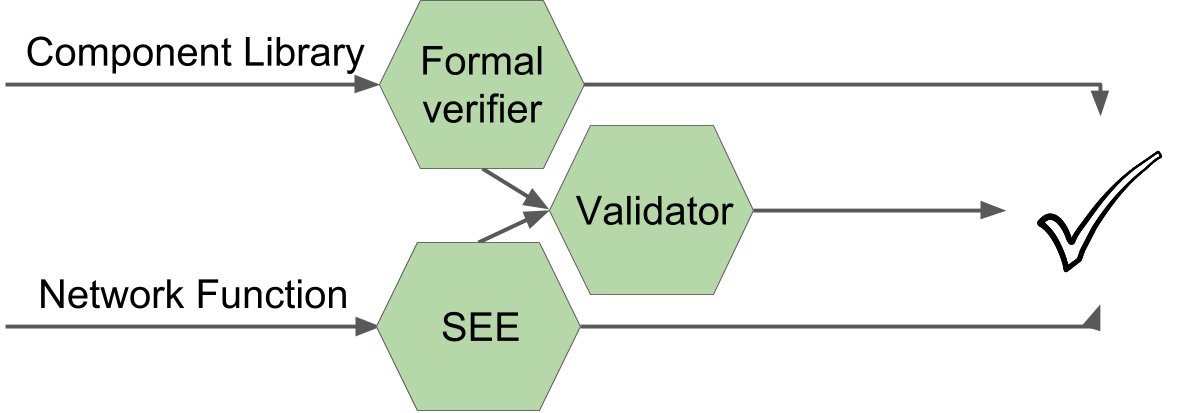
\includegraphics[width=\columnwidth]{figures/impl_overview.png}
    \caption{The Vigor tool chain for automatic verification.}
    \label{fig:arch}
\end{figure}

%---------------
\subsection{Speculative Verification}
\label{sec:our-approach}

Vigor views a network function as a combination of stateless application logic tied to components and data structures (collectively called ``components'') that are stateful, such as hash tables, arrays, least-prefix-match tables, etc. In the example of \S\ref{sec:solution-overview}, we encapsulated the \code{packets} array into the \code{ring} component. Singular variables of course need not be abstracted away, just large or variable-sized structures potentially accessed with symbolic indexes. The role of the library is to group stateful components into a unit that can be formally verified {\em once} an then {\em reused} across all NFs---we can view the Vigor library as a domain-specific extension of the C language. This makes sense because there is a relatively low number of components needed to support a wide range of NFs. Figure~ \ref{fig:algo} summarizes how Vigor works.

\begin{figure}[]
    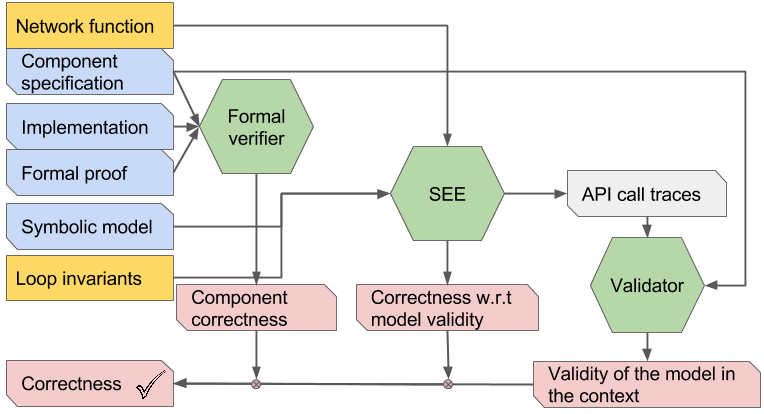
\includegraphics[width=\columnwidth]{figures/vigor_algorithm.png}
    \caption{The Vigor verification workflow. Rectangles represent data, hexagons are the Vigor tools, and arrows indicate the flow of data.}
    \label{fig:algo}
\end{figure}

It is feasible for NF developers to develop verified components and add them to the library. However, this requires a fair amount of verification expertise: formally specify the component interface, implement it in a way that can be verified but also has good performance, then produce a mechanically checkable proof, write one or more symbolic models for it, and finally a plug-in for the Validator. Vigor therefore adopts a usage model in which the vast majority of NF developers just use the components in the Vigor library and run Vigor to prove (or debug) their code.

%We had to find our own way to support high level data structures in SE, because the popular approach does not suit our goal. Many systems based on SE extend the target language with specification syntax allowing developers to formulate complex conditions. For instance, Frama-C/Value~\cite{kirchner2015frama} and VeriFast~\cite{jacobs2008verifast} use their own abstract specification language. We strive to make the verification simple and automated, but unfortunately current state of the art systems cannot reason automatically in such sophisticated terms and require manual small-step derivations. Developers end up spending more effort on the correctness proof than on the code itself.

%We explore an alternative way: 

For each component of the library, Vigor provides several symbolic models. A model is a concise over-approximating abstraction of how the specific component behaves when invoked by NF code. A good model has very little state. When symbolically executing an NF, the SEE uses one model for each component, and explores all execution paths through the NF together with the models. If every execution path has the desired property, then the NF has that property at all times. Since models are relatively easy to write, it is conceivable for NF developers to also write symbolic models.

A desired property is formulated as an assert. ``No division by zero''  is stated as an assert that the denominator is non-zero; ``safe memory access'' is stated as an assert that accessed memory is ``owned'' by the accessor. More details appear in \S\ref{sec:properties}. If a symbolically executed code path completes without any assert failing, we say the execution path was successful.

For each execution path, the Vigor SEE produces a trace of how the NF code interacted with the components it uses (we define these traces formally in \S\ref{sec:model-validation-criteria}). This is  {\em speculative} in that we don't have proof that the models are accurate abstractions of the components. The question the Validator answers is whether these traces are consistent with the formal specs of the components, i.e., could the interaction the NF code had with the model have been a legitimate interaction with an implementation of the component's specification. This is a weaker property than the model being a correct abstraction of the component, but it is sufficient for our purposes.

Of course, execution paths may not always succeed during SE. While this may be indicative of a bug in the NF, it could also be simply because the model is too approximate. For example, in \S\ref{sec:solution-overview} a model of \code{ring_empty} may be as simple as randomly returning true or false---for some NF code, this behavior could crash it, if it assumes \code{ring_empty} to return false right after pushing an element. A different model, however, keeps a counter of how many elements are in the ring, and makes \code{ring_empty} return true only when this counter is zero. The above NF code would not crash with this model; on the downside, the more stateful model makes SE take longer. Therefore, Vigor starts with the least-state models, and tries alternates until it either finds a model with which SE succeeds on all paths or not.

If Vigor does not find any symbolic model for which all execution paths through the NF code succeed, then it points the developers to the places where the properties fail to hold, and helps the debug.

%    \item The application developer provides loop invariants for long/unbounded loops (e.g. event loop in the example). The invariants are mostly a conjunction of the corresponding invariants for the symbolic models, but they are likely to have an application specific part.


% a number of speculative assumptions that we believe will hold for the real implementations. In the example above some of these assumptions are: ``the \code{ring_empty} function may return either 0 or 1'', ``if the \code{ring_pop_front} returns success the popped packet’s port will never be equal to 9'', and ``\code{ring_push_back} never crashes''.

% ^^^ do not forget to uncomment the references together with the figure
% \begin{figure}[h]
%     \centering
%     \def\svgwidth{\columnwidth}
%     \input{pie.pdf_tex}
%     \caption{Our conceptual division of the code into stateless and stateful parts with a strict interface between them.}
%     \label{fig:pie}
% \end{figure}

%-----------------
\subsection{Assumptions}
\label{sec:assumptions}

Our approach makes several assumptions. First, we assume that our symbolic models are over-approximations of the environment in which the NF runs (network stack, OS, etc.). In devising these models, we aim to include every possible behavior, but the absence of a formal specification of the environment makes it impossible to validate the models. Second, our guarantees rely on the hardware running the software dataplane correctly. Third, we assume the compiler implements the same language semantics employed by our tools (e.g., same byte length for C primitive types).

Thus, the trusted computing base for a Vigor-verified NF consists of the compiler, the Vigor tool chain (including its formal verification engine and SEE), the network stack, device drivers, OS kernel, BIOS, and hardware.

% We distinguish of the verified component library from development of an application using this library. These two activities require different skills and ideally should be done by different people.

% This paper proposes the following approach expressed in a number of steps. We use three tools: ``SE verifier'' stands for our SEE, ``formal verifier'' is our formal verification proof checker and assistant and a ``validator'' --- the tool that validates legitimacy and exhaustiveness of the model behaviour post factum. We differentiate human work between two developers: a component developer and an application developer. During the development of our NAT box they were the same person.

%------------------------------
\subsection{Handling pointers}
\label{sec:handling-pointers}

Pointers are the soul of the C language---they embody the power and the danger of low-level systems code. A NF focused on performance can not avoid them. We embrace them and support the most used idioms in our tool.

An important choice is the memory allocation strategy. Dynamic allocation offers more flexibility but incurs performance penalties. Static allocation should be preferred because it allows better control over layout, making it possible to optimize for cache and same the allocation overhead at runtime. However static allocation reduces flexibility, e.g. it fixes the component capacity at the compile time.

Among all the pointers appearing in the execution context, only the pointers crossing API boundary are important for the model validation. We divide these pointer into two kinds: argument pointers and return pointers.

An argument pointer may be either:
\begin{itemize}
    \item The address of the component state structure. It is an equivalent of ``this'' pointer for C++/Java or ``self'' reference for Rust/Python. We do not inspect the memory by such pointers, we only note the aliasing between them. The component owns this memory and only the formally verified code can access it.
    \item Output parameter. The application owns this memory. Therefore we have to trace the evolution of the pointee value. The pointee value before the call, which we trace as the function input, and the pointee value after the call, which goes to the function output. A special case of output pointer is a double pointer to the component state structure (X** p), set by the component allocation function. The app then owns the pointee (*p), and the SE verifier traces it, but the pointee of the pointee (**p) is the component internal state, so no need to trace it. We currently do not support other cases of double or deeper pointers (e.g. an output parameter to be set to point to a piece of the internal state).
\end{itemize}

A return pointer for our components always points to a piece of the internal state (e.g. an array cell). We trace the pointee and also make sure the application does not access it when the component regains the ownership.

%--------------------
\subsection{Property Formulation}
\label{sec:properties}

Vigor can verify any property that can be stated as a safety property, i.e., formulated as an \code{assert} condition. This includes various sources of crashes (dereferencing a null pointer, reading from an unmapped memory page, dividing by zero, etc.) as well as several classes of security bugs related to memory safety (writing to unallocated memory, writing to the wrong memory object, use-after-free, double-free, etc.) and related to integer operations (e.g., integer overflow).

When symbolically executing a code path, the SEE checks whether any asserts fail.

To check for memory leaks (or leaked resources in general) is a bit more complicated, because that is a global property. Vigor therefore must keep track of memory ownership. In the application logic we forbid dynamic memory allocation, and all allocated memory is controlled in the library, thereby giving the formal verifier explicit visibility into memory ownership. The temporary pointer access control enables the SE verifier to ensure the application returns all the memory chunks taken from a component and never accesses them after that.

Vigor does not specifically deal with semantic properties (e.g., dropping a packet, using an incorrect MAC address as a destination), but many of these properties can be formulated by NF developers as \code{assert} statements in their code. Vigor will then determine whether those \code{assert}s hold on all paths.

%----------------------
\subsection{Validating a Symbolic Model}
\label{sec:model-validation-criteria}

To validate a model behavior under certain circumstances means to ensure the behavior agrees with the specification, or is more relaxed (i.e., admits more behaviors than the spec). Suppose that, for the input \(I\) to the prefix of an execution trace (a ``run''), the specification produces the output $O_s$, and the model produces the case output \(O_m\). Then the model is valid iff for all call sequences performed during the exhaustive SE, \(O_m\) contains \(O_s\).

More formally:
\begin{enumerate}
    \item \(C\): A call sequence, or a run (\(C=Ci+Co\)) consists of a run input and run output. It summarizes a particular interaction scenario with the model. It consists of the calls to component API functions (with function names, arguments and return values), and leaves out all other details like other calls or unrelated path conditions.
    \item \(Ci\): The run input (\(Ci = <Fi,Fo>i=0..n-1 + Fin\)) is a set of: function names, function inputs(\(Fi\)) for all the functions in the sequence and function outputs(\(Fo\)) for all but the last call.
    \item \(Co\): The run output (\(Co = Fon\)) is the output of the last API function call in the sequence.
    \item \(Fi\): The function input (\(Fi = fun\_name + args + arg\_pointee\_vals_before + constraints\)) consists of the function arguments (possibly symbolic), and constraints bounding these arguments (specifically, the transitive closure of all the constraints involving the symbols mentioned in the formulas for the arguments). For a pointer argument (which must point to a concrete address --- practical limitation), the pointee must be considered according to the \S\ref{sec:handling-pointers}. We use the numerical value of the pointer to detect aliasing between the variables, and then throw it away, since we forbid pointer comparison anyway.
    \item \(Fo\): The function output (\(Fo = ret\_val + pointee\_vals\_after + constraints\)) is its return value and the pointee values for the output pointer arguments, as well as the constraints for all the symbols involved (transitive closure, same as above).
\end{enumerate}

Let us represent the formal specification and the symbolic model total states by large sets. A total state consists of variables V, bound by logical formulas F. So, the specification and model total states are:
\[
\{V_s : F_s(V_s)\} and \{V_m : F_m(V_m)\}
\]
The output is then simply a projection of the corresponding state. The projection (P) gives the output variables (return value and output pointers of the tip call): 
\[
OV_s = P_s(V_s): OV_m = P_m(V_m).
\]

\begin{figure}[h]
    \centering
    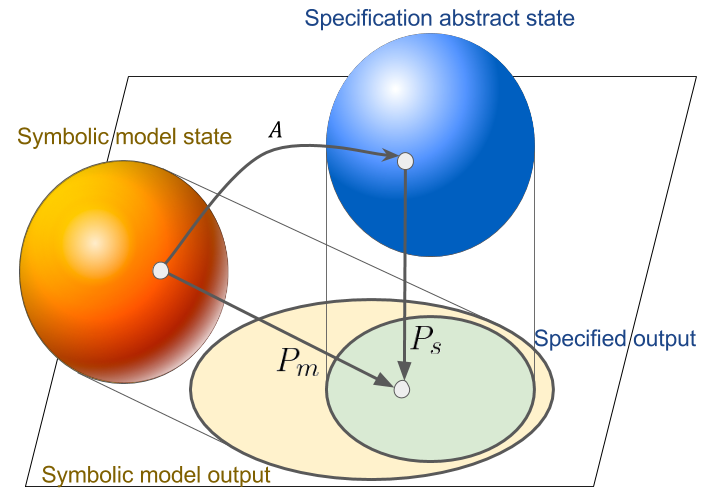
\includegraphics[width=\columnwidth]{figures/projections.png}
    \caption{The outputs \(O_m, O_s\) represented as projections of the total formal specification and model states.}
    \label{projections}
\end{figure}

With the introduced definitions, the following formulas define the outputs:
\[
O_s = \{P_s(V_s): \forall V_s F_s(V_s)\} \\
O_m = \{P_m(V_m) : \forall V_m F_m(V_m)\}
\]
Then, the model exhibits all the specified behaviours (and may be some more) iff \(O_s \in O_m\), or: 
\[
\forall V_s : F_s(V_s) \exists V_m : F_m (V_m) \cap P_s(V_s) = P_m(V_m)
\]
This formula in general is too difficult for the existing SMT solvers because of the quantifier. However, due to similarities in the model and the specification it is easy to find appropriate values for \(V_m\) --- they happen to be some values from Vs. Let us call this assignment \(A\). \(A\) by construction satisfies the equality \(P_s(V_s)=P_m(A(V_s))\). So the condition becomes:
\[
\forall V_s : F_s(V_s) \rightarrow F_m(A(V_s))
\]
  --- a typical validity query, which we pass  to an SMT solver.
  
This validation criteria guarantees that the formally verified implementation will never do anything that the model did not explore during verification. So each possible behaviour of the real execution (and may be some extra) was checked during the SE, and it is 1) allowed by the specification and 2) does not cause the application code to crash.



\subsection{Algorithmic Requirements}
\label{sec:algorithmic-requirements}

For a NF to be verifiable by Vigor, it must fulfill several requirements. These are fully aligned with best practices in developing NFs.

First, the application must contain no deep recursion and only use well structured loops. For long or unbounded loops, a developer must supply an invariant. Most NFs naturally satisfy this requirement due to performance considerations.

Second, program state must be encapsulated in a set of formally specified components (e.g., port allocator) or data structures (e.g., hashtable). Vigor uses the component API as a boundary between the code that is automatically verified using SE and the code that is manually verified.% (Figure~\ref{fig:pie}).

Third, there must be a well defined OS interface. As it is infeasible to symbolically execute the whole OS, the SEE stops at the OS interface boundary. Behind this interface we trust the correct implementation and we use symbolic models of the OS API functions for SE. It is conceivable to use a verified OS kernel, like SeL4~\cite{klein2009sel4}, and thus have a fully verified stack. 
    
Finally, the NF must implement a classic event loop; most NFs already do so. For Vigor specifically, there must be a single infinite loop, with each iteration dedicated to processing a single event (an incoming packet). Within each iteration, the sequence of interactions between the code and the library components and the OS must be relatively short --- the complexity of models and the amount of symbolic state are often proportional to the length of the API call sequence it needs to support.

\subsection{Language Restrictions}
\label{sec:language-restrictions}

When writing NFs to be verified with Vigor, developers are free to use C. However, we impose a few restrictions that ensure good isolation between application code and the library components: We require that the component-related memory be accessed only through the library API. There should be no pointer comparisons except for equality --- the C99 standard anyway prohibits most pointer comparisons, and we extend this restriction in order to better isolate the component implementation from the code that uses it. Finally, pointer accesses must be both domain-limited and time-bounded: certain pointers may access only predefined range (i.e. a single unit of the declared type) and only on a restricted segment of the execution, between the corresponding API calls.
    
These restrictions do not apply to the formally verified component library. 

% \subsection{Component Design Choice}

% A component designer faces a choice between conciseness and performance. Low expressive power of C forces the component developer to implement an abstraction either through typeless pointers or macros. Pointer implementation introduces an extra dereference, which may hurt performance. Macros are a zero cost abstraction. They perform better as they avoid extra pointer dereference and inline-friendly. Unfortunately, they hurt conciseness and readability of the code. In the long stretch a generics language extension such as C++99 templates could alleviate this trade-off.

\section{Implementation}
\label{sec:implementation}

In this section we describe the prototypes that embody the ideas presented in the previous section. We then use these prototypes to evaluate Vigor on the development of a NAT middlebox, described in \S\ref{sec:evaluation}.

\subsection{Vigor Tool Chain}

To assess the practicality of Vigor technique, we implemented the three tools described in the section~\ref{sec:our-approach}. The SEE is responsible for the application verification, the Formal Verifier checks correctness of the components’ implementation in the library, and the Validator ensures the two verifiers agree on the component APIs used.

\paragraph{SE verifier} We built our verifier for speculative SE by modifying an open source C/C++ SEE Klee~\cite{cadar2008klee}. By default Klee terminates execution paths that are too long or take too much memory. We disabled this feature to ensure it explores all the paths. We also extended KLee with three new features:
Partial loop invariant support. The analysis finds automatically the variables that may change in the loop, and havocs them. Currently, a developer have to manually insert the assertions and assumptions according to the loop invariant definition.
Dynamic pointer access control. The patch provides primitive intrinsics that allow a component developer to open and close access to a pointer between the API calls.
API call sequence dump. This patch summarizes each control path in the program extracting the component API calls and dumps them for the Validator.

\paragraph{Formal verifier} Our verifier is essentially VeriFast~\cite{jacobs2008verifast} extended with the ability to export the abstract state (\(O_s\)) for the Validator. Specifically we export the accumulated conditions for the output variables at the end of the API calls sequence.

\paragraph{Validator} We wrote this third tool completely from scratch. Validator independently analyzes each API calls sequence. We exploit the data parallelism using GNU parallel tool~\cite{Tange2011a}. For each API call sequence in the Klee dump, Validator first transforms it into VeriFast task. A VeriFast task is essentially a C source file, containing the sequence of calls. The Validator enriches the sequence with:
\begin{itemize}
    \item Symbolic variables used in the sequence.
    \item The constraints that form the sequence context.
    \item Lemmas to help formal verification.
\end{itemize}
Next, it runs VeriFast to check that the specification permits this particular sequence of calls under the provided constraints. Finally, the Validator imports the specification output state \(O_s\) and checks the inclusion of the specification state \(O_s\) to the model state \(O_m\) using Z3~\cite{de2008z3} SMT solver (see Section~\ref{sec:model-validation-criteria}).

Figure~\ref{fig:validator} shows the data flow between the Validator elements.

\begin{figure}[h]
    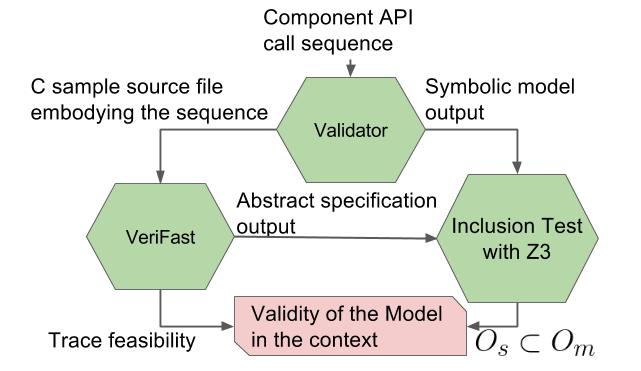
\includegraphics[width=\columnwidth]{figures/validator.png}
    \caption{The internal Validator dataflow.}
    \label{fig:validator}
\end{figure}


\subsection{Verified Component Library}

For our Vigor library prototype, we implemented four stateful components. These are sufficient to develop the NAT middlebox of \S\ref{sec:evaluation}: A hash map keeps current flows, and allows lookup by two keys corresponding to the packets coming from internal and external interfaces; the Port allocator is responsible for allocating new ports and expiring inactive entries; the Batcher allows batch processing, keeping outbound packets until the NIC is ready to send them; and the Static Array instances keep various configuration values. We are careful in how we abstract components like the Static Array, because NFs are expected to access them on hot paths, and so it is important that the data reside in the processor cache.

\paragraph{Hash Map}

We implement a two-key hash map using three parts: integer indexed array of flows and two single-key hash maps. The array stores flows together with the keys. The hash maps internally are fixed size arrays of tuples $<$busy-bit, key-hash, key-ptr, flow-index$>$:
\begin{itemize}
    \item Key-hash is the value of the hash function for the key.
    \item Key-ptr is the pointer to the full key for precise comparison.
    \item Value-index is the index in the array of values.
    \item Busy-bit flags the tuples that are not garbage.
\end{itemize}


Flow insertion linearly searches a free cell (with busy-bit = 0) from an index equal to the hash of the corresponding key. To insert a flow, user must also supply an unused index. We use port allocator to allocate these indexes.

Flow search and removal also starts from the hash-induced index looks for a cell with the same hash, with confirmation by a total equality of the stored and searched keys.

This implementation is not efficient for some cases. For instance, if the flow is not present in the table, the algorithm will traverse the whole table and the search time will be proportional to the capacity.

To address this inefficiency, we optimize the single-key maps. We add another bit into the tuple. These bits group cells into hash-collision chains, and the map searches for a flow only across that chain, not across the entire table. Unfortunately, we did not yet verify the optimized implementation. We estimate re-verification to take about half of the initial verification effort (see section~\ref{sec:efficiency})

A hash map is a widely used data structure. It allows to store and retrieve entries by arbitrary complex keys. Such functions as L2 switching, ACL filtering, IPS, etc. all use hash tables.

\paragraph{Port Allocator}

Port allocator keeps two chains \emph{alloc} and \emph{free} packed into an array. The size of the array equal to the port range available to allocator, and each cell corresponds to a port to be allocated. \emph{Alloc} chain is a double linked list. It contains all the allocated ports with last access timestamps sorted by these timestamps. \emph{Free} chain is a single linked list. It keeps track of the available ports.

All operations take constant time, and only manipulate the cells of the array. Allocate operation moves head of the free chain to the head of the alloc chain. Access moves the element from the middle of alloc chain to the head. Expire takes the tail element from the alloc chain and moves it to the head of the free chain.

The port allocator is essentially a number allocator from a predefined range. Constant time allocation and expiration makes it a basic component for any application that manages resources in run time, such as L2 switch or L3 router.

\paragraph{Batcher}

Batcher is an array with a counter. It allows to store elements one by one (up to a preset capacity), and to release them all at once. Almost every DPDK example uses a batcher. It is necessary to achieve high throughput, because NICs work better on batches, rather than on individual packets. 

\paragraph{Static Array}

Every DPDK example uses multiple static arrays for various configuration parameters, counters and other statistics. Our static array is a thin wrapper around a regular C array. This wrapper adds zero overhead, but enables our tool-chain to control access to the array and to substitute the whole array with just a couple of bytes during SE.

%===================

\section{Evaluation}

\label{sec:evaluation}

In this section we answer three questions:
\begin{enumerate}
    \item Is our approach effective at verifying real-world stateful NFs? In \S\ref{sec:effectiveness} we provide a qualitative answer to this question for a DPDK-based NAT middlebox.
    \item How efficient is our approach in terms of human and compute effort (\S\ref{sec:efficiency})?
    \item Is the performance of the verified NAT box good enough for practical real-world use by sysadmins and network operators (\S\ref{sec:performance})?
    %\item What are the trade-offs inherent to Vigor, and how do they impact verifiability and performance? In \S\ref{sec:tradeoffs} we give the reader a deeper understanding on how the various parts of the technique contribute to its scalability and cost.
\end{enumerate}

As a proof of concept, we implemented and verified \vignat, a NAT middlebox based on the DPDK framework~\cite{intel2014data}. We use NAT to refer specifically to Dynamic Source Network Address-Port Translation~\cite{rfc3022}. We reused boilerplate code from the DPDK L3 forwarding example. \vignat has 1,175 LOC, and it links with the Vigor library that has an additional 941 LOC. \vignat supports TCP and UDP packet forwarding with dynamic source address--port translation between multiple internal and one external interfaces. It supports connection initiation from an internal interface and refuses connections from the external one. It supports concurrent flows up to a configurable maximum number; flows expire after a configurable period of inactivity.

% The biggest difference of our application code from a usual code you can see in network applications is array access. To get an element from our Static Array component, due to our memory ownership technique, a developer have to explicitly borrow it through API call and then return the borrowed element to access another one.

Our evaluation uses two versions of this NAT box. During our experiments we discovered a silly performance bug in our hash table implementation that led to excessive hash collisions under certain circumstances. We fixed it, but did not complete the re-verification by the submission deadline. We therefore report results for both \vignata (100\% verified but slow) and \vignatb (verified, except for the hash table).

%---------------------------
\subsection{Vigor's Effectiveness}
\label{sec:effectiveness}

The ultimate goal of our work is to give operators the confidence that software-based NFs will not undermine the robustness and security of their network. It took about 12 minutes on a laptop for Vigor to prove that \vignat is free of crashes, free of memory leaks, free of memory overflows, and free of integer overflows. We verified \vignat only for one internal and one external interface, but do not foresee any challenges in doing so for multiple interfaces. 

Beyond merely providing a binary yes/no answer to the question of whether an NF has a given property or not, Vigor also helps developers find those corner cases that impede the proof. There are three classes of bugs that Vigor uncovers in the verification process, and as the citations show, these appeared in the released Open vSwitch and DPDK code:
\begin{enumerate}

    \item Security vulnerabilities~\cite{bug:ovs-uaf, bug:dpdk-uaf1, bug:dpdk-uaf2, bug:ovs-faf, bug:ovs-overflow, bug:dpdk-overflow1, bug:dpdk-overflow2, bug:ovs-int-overflow, bug:dpdk-int-overflow} in the form of memory overflows or integer overflows. These can enable an attacker to gain remote control of the middlebox.
    
    \item Crashes~\cite{bug:ovs-0ptr, bug:dpdk-0ptr1, bug:dpdk-0ptr2, bug:dpdk-0ptr3} destabilize the network. Furthermore, many of these can be triggered by a remote attacker with a carefully crafted packet (e.g., trigger a bad pointer dereference or a division by zero), thereby opening up the middlebox to denial-of-service attacks.

    \item Memory leaks~\cite{bug:ovs-mem-leak1, bug:ovs-mem-leak2, bug:ovs-mem-leak3, bug:ovs-mem-leak4, bug:dpdk-mem-leak1, bug:dpdk-mem-leak2} are often exploited for denial-of-service by exhausting the middlebox's memory. Vigor's memory ownership model makes them both easy to find and to debug.

\end{enumerate}

Vigor does not support today proving concurrency properties or higher level semantic properties. Nevertheless, we consider the verifiable absence of low-level flaws to be a solid step toward complete verification.

%---------------------------
\subsection{Efficiency of Using Vigor}
\label{sec:efficiency}

A key question when using Vigor is how much longer does it take a developer to produce verified code vs. non-verified, and how much harder is it.  Another question is how much effort it takes to develop and verify the component library, but that effort gets amortized across many uses and is therefore less important.

\vignat's 1,175 LOC require about 30 lines of developer annotations (3\% overhead) in the form of loop invariants and loop labels like \code{LOOP(1)} in \S\ref{sec:solution-overview}). Static analysis can infer all the other information needed for the proofs. In our current Vigor prototype we have not implemented this static analysis, and so our \vignat prototype has 176 lines of annotations (15\% overhead)in the form of C structure layout description, conditional compilation constructs, etc. that make up for simple but unimplemented analyses in Vigor.

Our estimate is that it would take an NF developer about 1 week to develop and verify \vignat based on reading this paper (in particular \S\ref{sec:algorithmic-requirements} and \S\ref{sec:language-restrictions}). Our own development time is less representative, both because of our understanding of the system and the fact that we co-developed Vigor with \vignat.

Once the code is developed and annotated, verification is fast. On an Ubuntu 16.04 Linux laptop with an Intel I7-6600U CPU and 16GB LPDDR3 RAM, exhaustive SE of \vignat takes 2 minutes and 650 MB of RAM, and the Validator takes 10 minutes to validate the 700 call sequences that result from SE. Verification of the library's correctness proof takes 15 seconds.

\medskip 

Developing and verifying the library took about 5 person-weeks, not counting our learning curve and various setbacks. Detailed data appears in Appendix B.

Table~\ref{tab:loc} shows the size of each of the library's four components.  As expected, the formal specification and proof dwarf by a 10-20$\times$ margin the implementation.  This is why we consider Vigor's design---using SE for NF code on the one hand, and heavy verification for the reusable library on the other hand---to provide a favorable balance for real-world NF development.  The symbolic model and the validator plug-in are more concise than the component implementation, which makes it feasible to provide several of them for each component, to suit different usage patterns.


\begin{table*}[h!]
\centering
\caption{Size (in LOC) of the parts required to develop and prove each  library component and data structure.}
\label{tab:loc}
\begin{tabular}{lllllll}
\hline
  Component             & Interface & Implementation & Formal spec & Symbolic model & Proof & Validator plug-in \\ \hline
{\bf Hash Map}        & 29         & 688            & 596                  & 281            & 4,078         & 450              \\
{\bf Port Allocator} & 22         & 210            & 310                  & 95             & 4,439         & 129              \\
{\bf Static Array}   & 8          & 15             & 31                   & 145            & 155          & 39               \\
{\bf Batcher}        & 22         & 28             & 27                   & 60             & 65           & 23               \\ \hline
\end{tabular}
\end{table*}

%---------------------------
\subsection{\vignat Performance}
\label{sec:performance}

In this section we address the question of whether verifiability comes at the price of performance. We evaluate \vignat's forwarding throughput and latency, comparing it to a NAT based on  NetFilter~\cite{boye2013netfilter}, which is widespread and used in all the Linux-based home and small-enterprise routers. We set up the NetFilter masquerade rules as shown in Appendix A, and we tune the Linux kernel for optimal performance as described in~\cite{nf-testing}. We label it {\em LinuxNAT} in our plots.

As mentioned earlier, we report on two versions of our NAT: \vignata has a performance bug in the hash table, whereas \vignatb does not, but its hash table is not yet verified. We configure both to have a maximum capacity of 61,000 flows. We use three identical machines, each a 32-core Intel Xeon E5-2667 v2 @ 3.30GHz with 32GB RAM with i350 1 Gbps DPDK-compatible NICs. 

% The throughput results are stable, so we do not collect statistical significance. However latency varies noticeably and we measure repeat the experiment ten times to reveal the variability.

%-------------------------
\paragraph{Throughput.}

We set up two nodes in the topology shown in Figure~\ref{fig:throughput-setup}, as per RFC 2647~\cite{rfc2544}: a tester machine connects to the middlebox over two interfaces. We use \code{DPDK-Pktgen}, a high-performance traffic generator; it sends packets through {\em outbound} and counts them on the {\em inbound} interface. It assigns each packet a port from a given range to generate the corresponding number of distinct flows. We run 40-second measurement intervals.

\begin{figure}[h!]
    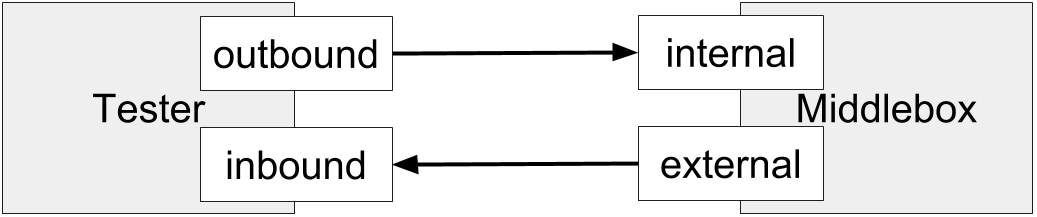
\includegraphics[width=\columnwidth]{figures/throughput_setup.png}
    \caption{Network topology for throughput experiment.}
    \label{fig:throughput-setup}
\end{figure}

In Figure~\ref{fig:throughput-overall} we show the maximum packet rate achieved with a maximum of 1\% packet loss, for different numbers of concurrent flows. At the outset, \vignat outperforms LinuxNAT; this is in no way related to Vigor but rather is due to DPDK and to LinuxNAT being interrupt driven. % Our prototype is not optimized either, but the fact that it uses DPDK makes it much more efficient. %; compared to a trivial DPDK application that merely forwards packets, \vignat does not add

\begin{figure}[]
    \centering
    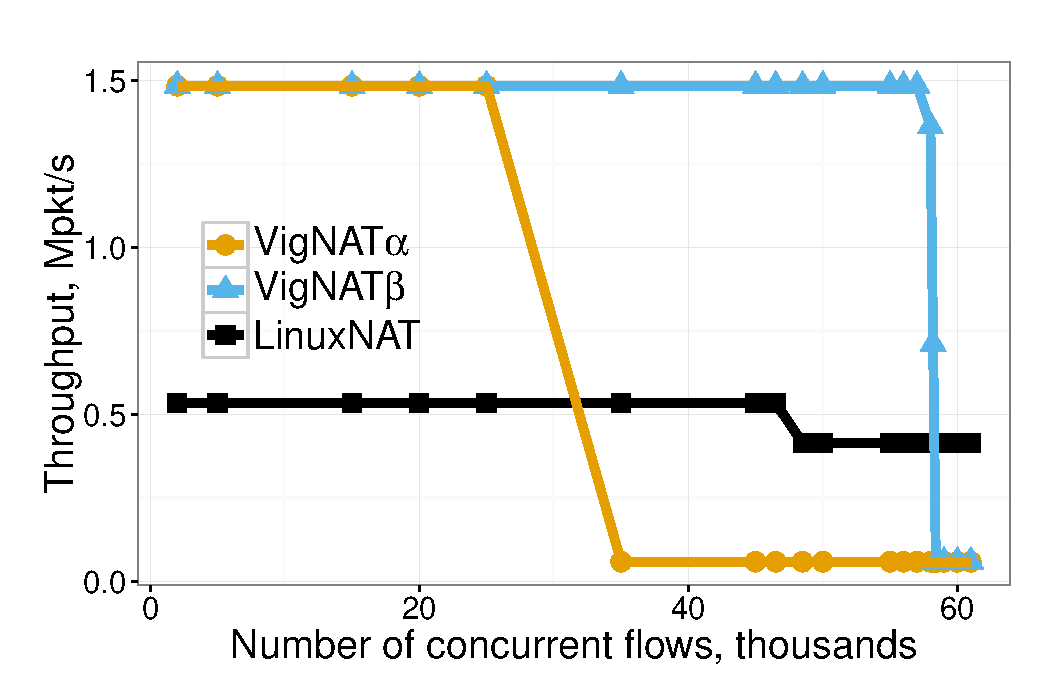
\includegraphics[width=0.5\textwidth]{plots/brpt.pdf}
    \caption{Throughput as a function of the number of concurrent flows, with maximum 1\% loss rate.}
    \label{fig:throughput-overall}
\end{figure}

\vignata does well up until $\approx$28K connections, at which point it collapses due to the performance bug. In contrast, \vignatb sticks to the zero-loss line up until $\approx$59K connections, at which point our 61K-entry hashtable experiences too many collisions to keep up---increasing the size of the hash table would move this point further to the right.

To zoom in on what happens around those two inflection points, we plot two throughput graphs. Figure~\ref{fig:throughput-27900} shows what happens for 27,800 concurrent flows: the hash collision bug in \vignata starts causing it to grind to a halt at specific send rates; this behavior gets rapidly worse as the number of concurrent flows increases. Figure~\ref{fig:throughput-59k} shows what happens for 59,000 concurrent flows: \vignatb's flow table fills to 95\% and thus slows down, starting to perform comparably to LinuxNAT on average, but with significant jitter. As the number of flows increases, \vignatb slows down further. % Reducing jitter is part of future work.


\begin{figure}[]
    \centering
    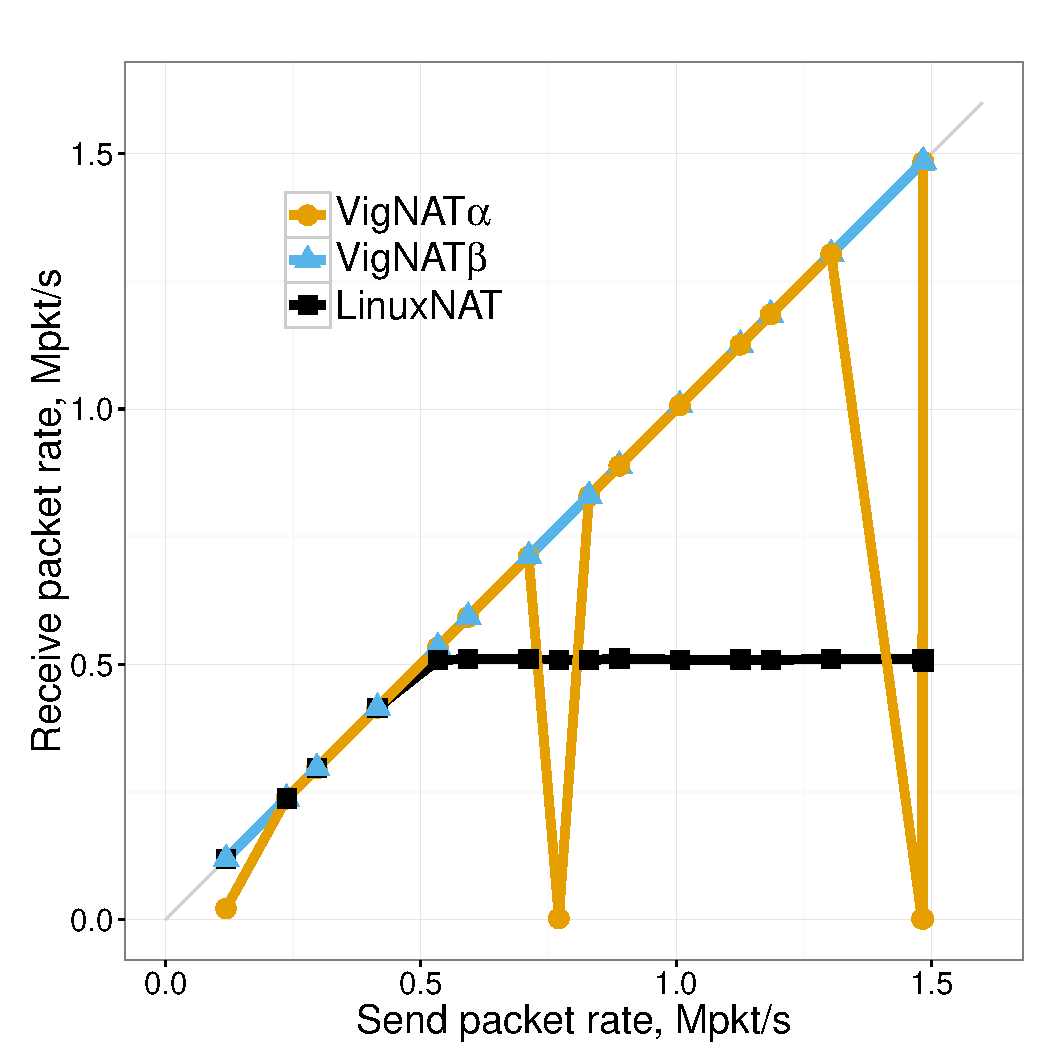
\includegraphics[width=0.5\textwidth]{plots/rt27900.pdf}
    \caption{Packet rates for 27,900 concurrent flows.}
    \label{fig:throughput-27900}
\end{figure}


\begin{figure}[]
    \centering
    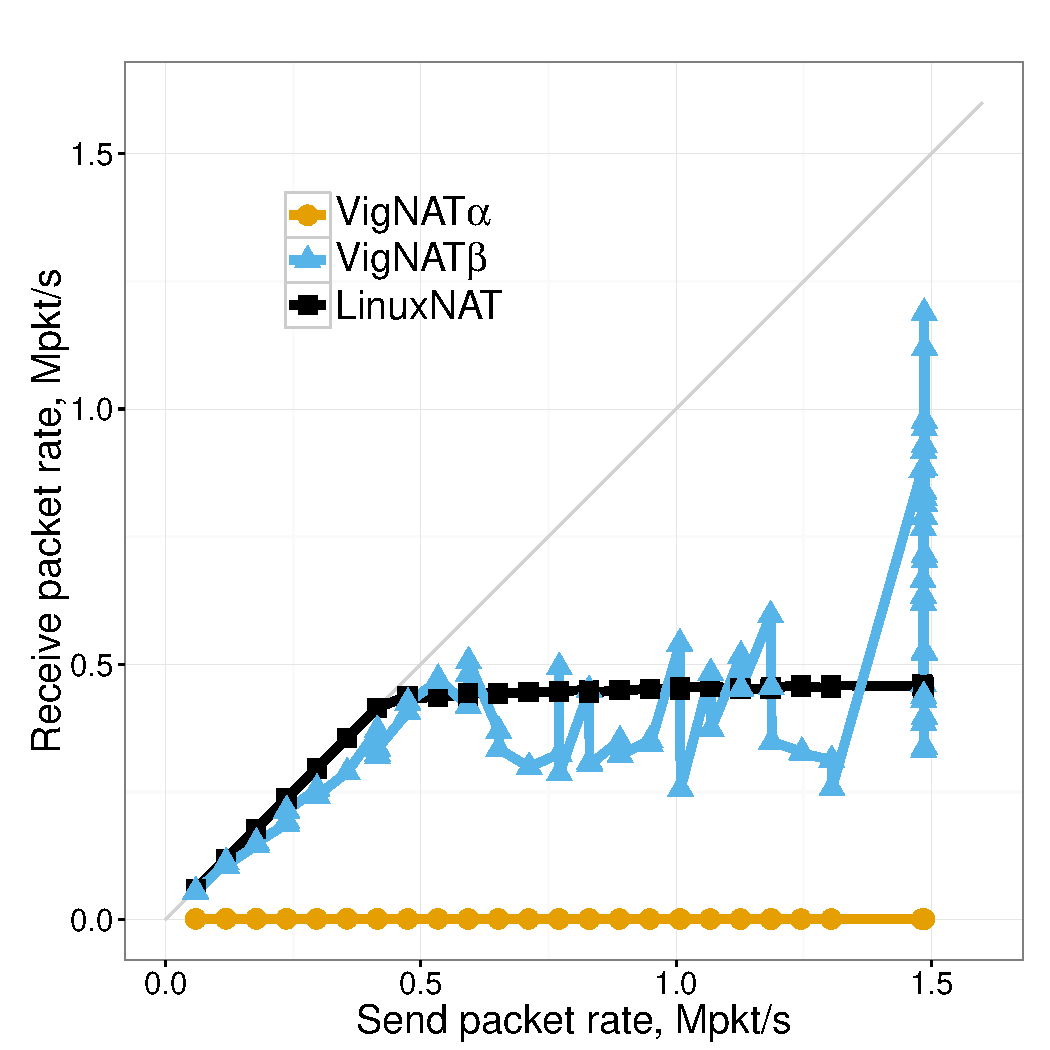
\includegraphics[width=0.5\textwidth]{plots/rt59k.pdf}
    \caption{Packet rates for 59,000 concurrent flows.}
    \label{fig:throughput-59k}
\end{figure}

%---------------
\paragraph{Latency}

To assess \vignat's latency characteristics, we use the network topology in Figure~\ref{fig:latency-setup}. We use separate ports on the tester for flow generation and latency sampling. We use again DPDK's \code{PktGen} for packet generation. We sample latency with netperf~\cite{jones1996netperf} \code{TCP_RR}, which measures the request-response delay to \code{netserver} and computes the average over 80 seconds.

\begin{figure}[h]
    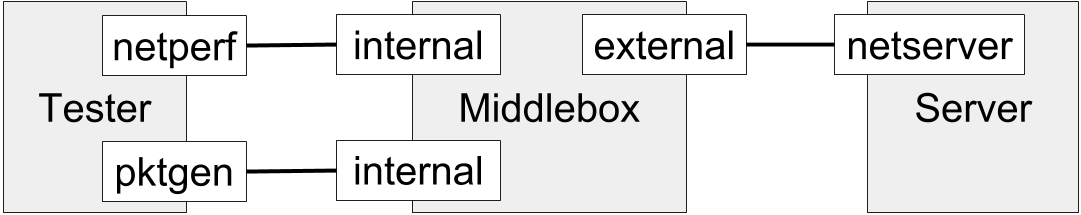
\includegraphics[width=\columnwidth]{figures/latency_setup.png}
    \caption{Network topology for latency measurements.}
    \label{fig:latency-setup}
\end{figure}

We also wrote a trivial DPDK application, derived from the DPDK l2fwd example~\cite{dpdk-l2fwd} which only forwards packets. To eliminate the routing overhead, we replaced L2 routing with a simple MAC address swap. This application is stateless and performs only a couple writes to the packet header, so we consider it the lowest possible latency one could achieve with DPDK; we label it {\em Plain forwarding} in our plots.

Figure~\ref{fig:latency-plot} shows one-way latency as the number of concurrent connections through the middlebox increases. The performance issue in \vignata causes its latency to increase with the number of flows, but \vignatb stays flat. There is increasing jitter as the number of flows increases, and investigating this is part of future work (we believe it's due to DPDK). \vignat has on average 23\% higher latency than LinuxNAT, but nevertheless stays under 111~$\mathrm{\mu sec}$, providing sufficient performance for many settings. Note that DPDK is designed to sustain high throughput, so it uses batching aggressively, which hurts latency---\vignat introduces a mere 5\% overhead compared to {\em Plain forwarding}.

\begin{figure}[h]
    \centering
    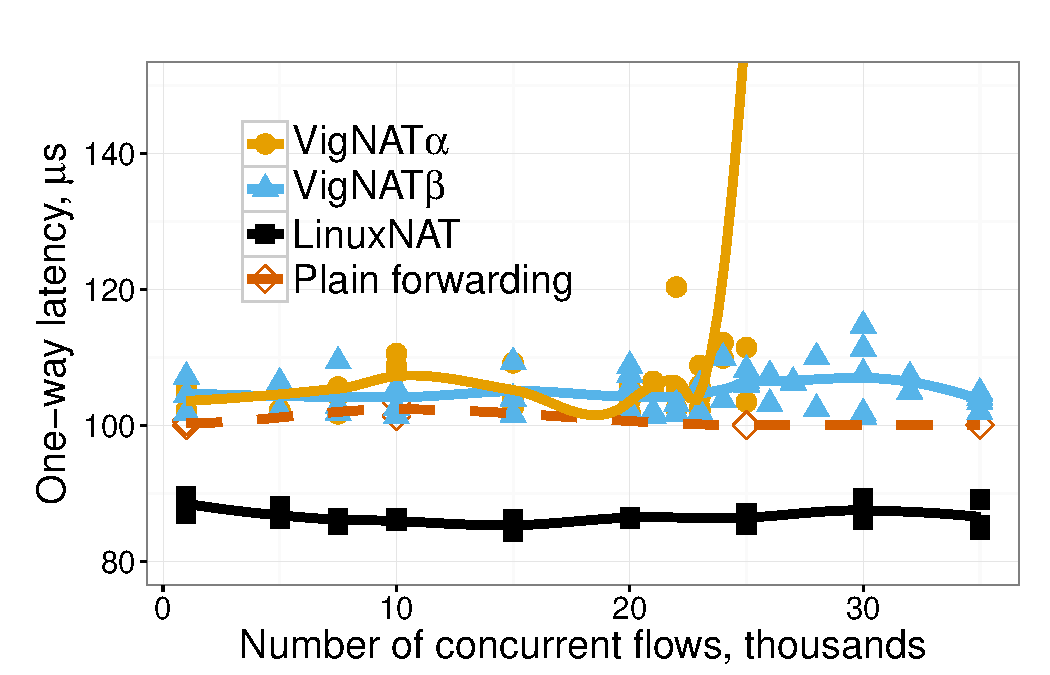
\includegraphics[width=0.5\textwidth]{plots/lat.pdf}
    \caption{Latency vs. number of concurrent flows.}
    \label{fig:latency-plot}
\end{figure}

%---------------
\bigskip 

If the reader believes our assertion that we can verify \vignatb's hash table in a few person-days, then the results in this section imply that developing a verified NAT middlebox does not come at the expense of performance. NF developer effort is relatively low, which makes this a practical approach. We therefore conclude that Vigor can succeed in its objective of enabling developers to productively write software-based data plane NFs that simultaneously meet the highest standards of reliability, security, and performance. 

\section{Limitations}

\label{sec:limitations}

Vigor's greatest limitation is that it is not fully automated yet. In particular, we expect NF developers have to write loop invariants for long and infinite loops. These loop invariants are essential to enabling scalable exhaustive SE with our modified KLEE. As mentioned before, coming up with these invariants for NF code is typically not difficult. Nevertheless, one of our immediate future work items is to leverage invariant induction techniques~\cite{perkins2004efficient, yang2004automatically} to automate at least part of this task.

Application developers may also encounter ``false positives'', i.e., Vigor fails to prove the desired property. As mentioned before, this can be due to the property indeed not holding, or because the symbolic models are too over-approximate. The NF developer can either develop their own more detailed model, or request the component library developers to provide a suitable model.

Besides the trusted computing base described in \S\ref{sec:assumptions}, Vigor relies on the NF developer to state correct invariants, as well as the library developers to correctly annotate the symbolic models with KLEE intrinsics (so that they produce correct traces). Finally, we trust the NF developer to not link their application with unverified components. If any of these assumptions fail to hold, Vigor cannot guarantee any properties.

With respect to our NAT use case, as already mentioned we have two versions, one of which is not fully verified (but will be shortly). Also, our NAT does not participate in any routing protocols; it needs an L3 router on each interface to dispatch the packets to the rest of the network. We supply the MAC addresses of these routers as a runtime argument to the NAT, and can not update it on-the-fly.

\section{Related Work}

\label{sec:related-work}

%In this section we review some of the similar projects undertaken in the past.

Dobrescu et al.~\cite{dobrescu2014software} analyzed modular NFs. They managed to analyze many stateless Click elements using exhaustive SE, and exploiting modularity and low cyclomatic complexity of such applications. However, their original approach is very limited in verification of stateful elements. In addition to crash freedom they managed to verify bounded execution and filtering properties. Doing this in Vigor for stateful NFs is future work.

SeL4~\cite{klein2009sel4}, CompCert~\cite{stewart2015compositional}, and FSCQ~\cite{chen2015using} show how to do functional verification of practical systems. All of them prove the semantics of the system. Unfortunately they all require the use of a high-level programming language and deep expertise in the verification domain, which is unacceptable for our problem.

Beringer et al~\cite{beringer2015verified} applied formal verification to an OpenSSL implementation, proving its functional correctness and cryptographic properties. They used certified tool chain, reducing trusted code base just to just a small CoQ proof checker core (~8k LOC). While it paves the road for formal verification towards real systems, it is not yet suitable as a common development practice.

SymNet~\cite{stoenescu2013symnet} uses SE to reason about whole network configuration with per-flow state. They do not verify the middle box implementations, instead parse the configuration files and use special models in place of the components. Their work naturally complements ours.

IronFleet~\cite{hawblitzel2015ironfleet} also aims for a verification of applications distributed over a network. They use a different approach, though. Habwlitzel et al develop IronFleet from scratch in Dafny --- a high level language with built-in verification support.

Others checked existing distributed systems. Pedrosa~\cite{pedrosa2015analysis} and Guerraoui~\cite{guerraoui2011model} explored the global state tree down to a certain depth. Guerrauoi et al. used a similar approach to ours: they made reasonable assumptions that simplify verification and validated the ones that turned out important.

CEGAR~\cite{clarke2000counterexample} is similar to our technique in the spirit of optimizing out the high effort/low return work. It only refines the models when given a clear evidence of the their insufficiency. Clarke at al. demonstrated a very generic approach. We focus on the networking domain, and exploit the features inaccessible for CEGAR, like the low number of data structures and simplicity of the application logic.

\section{Conclusion}

\label{sec:conclusion}

We presented a technique for proving properties of software NFs. We exploit the specifics of NFs to combine the benefits of symbolic execution with formal verification. Our experimental results demonstrate the practicality of the approach for the development of NAT box that is guaranteed to have no memory leaks, never crash, be free of certain security vulnerabilities, yet still performs on par with NetFilter. 


{\footnotesize \bibliographystyle{acm}
\bibliography{bibliography}}

\section*{Appendix A: NetFilter rules}

{\tt \small
\begin{verbatim}
iptables -t nat -A POSTROUTING -o eth0 -j MASQUERADE
iptables -A FORWARD -i eth0 -o eth1 -m state \
    --state NEW,RELATED,ESTABLISHED -j ACCEPT
iptables -A FORWARD -i eth0 -o eht1 -j ACCEPT
\end{verbatim}
}

\section*{Appendix B: Person-hours to verify \vignat}

Table~\ref{tab:man-hours} shows the number of person-hours spent to 

\begin{table*}[h!]
\centering
\caption{Developer person-hours spent on each component part in hours.}
\label{tab:man-hours}
\begin{tabular}{lllllll}
\hline
               & Interface design & Implementation & Formal spec & Symbolic model & Verification & Validator plug-in \\ \hline
Hash Map        & 2.5*       & 2*             & 4.5*                 & 5.5*           & 73.5         & 11.5             \\
Port Allocator & 1*         & 1.5*           & 3.5*                 & 1.5*           & 70           & 7.5              \\
Static Array   & 1.5        & 0.5            & 2.5                  & 2              & 6            & 2                \\
Batcher        & 1          & 0.2            & 0.5                  & 1              & 0.5          & 0.2              \\ \hline
\end{tabular}
\end{table*}


\end{document}
